% !TEX root = ../thesis.tex
% adjust noise level
% @author Tobias Wulf
%

\section{Anpassung des Rauschniveaus für Noisy-Observation}\label{sec:exp3}


\textbf{Zweck:} Das Experiment ist eine Fortsetzung zum \autoref{sec:exp2} und schaltet zusätzlich zur Trimmung der Kovarianzfunktion nach \autoref{alg:fminconopt} die äußere Modelloptimierung über das Rauschniveau $\sigma_n^2$ nach \autoref{alg:bayesopt} ein. Es dient primär zur weiteren Anpassung der Referenzwinkelanzahl und untersucht sekundär die Möglichkeit zur Winkelfehlerminimierung unter Berücksichtigung der gemachten Beobachtungen im \autoref{sec:exp2}. Ziel ist es hier, einen Kompromiss zu finden, bestehend aus brauchbarer Generalisierung und akzeptablen Winkelfehler bei möglichst geringer Referenzwinkelanzahl. Dafür werden für jeden Durchgang Modellverlust, absoluter mittlerer Winkelfehler sowie der maximale Winkelfehler auf eine volle Rotation mit $720$ Simulationswinkeln bei einer Auflösung von $\SI{0,5}{\degree}$ berechnet. Dafür wird wie in \autoref{sec:exp2} das Regressionsmodell für euklidischen Abstand nach \autoref{eq:de2innorm} und \autoref{eq:kfun} in beiden Varianten einmal als mittelwertfreies Modell und Mittelwert-unterstütztes Modell betrieben. Es wird der in \autoref{fig:timings-vs-errors} grün gekennzeichnete Bereich (1) näher untersucht.

\textbf{Durchführung:} Die Durchführung ist aus \autoref{sec:exp2} zu entnehmen. Änderungen in der Durchführung beziehen sich auf die Ausführungen zur Ermittlung der Berechnungszeit für eine Winkelvorhersage, diese ist durch die Berechnung der Modellverluste für Winkel ersetzt.

\textbf{Erzeugte Datensätze:} Es sind für das Experiment 24 Trainingsdatensätze mit unterschiedlicher Referenzwinkelanzahl und ein Testdatensatz erzeugt worden. Alle Datensätze korrespondieren in Position und Verkippung.

\textbf{Matlab-Skript:} compareNoiseOptAbility.m, siehe \autoref{mcode:comparenoiseoptability}.

\textbf{Abweichende Parameter von \autoref{tab:sim-params-exp}:}

\vspace{5mm}
\begin{table}[htp]
	\centering
	\resizebox{\textwidth}{!}{
		\begin{tabular}{l l c l}
			\toprule
			\textbf{Parametergruppe} & \textbf{Parameter} & \textbf{Wert}         & \textbf{Kurzbeschreibung}                  \\ \midrule
			TrainingOptions          & nAngles            & $\left[8:1:31\right]$ & Simulationswinkelanzahl inkrementiert um 1 \\ \hline
			GPROptions               & kernel             & 'QFCAPX'              & Indikator für zweite Kernel-Variante       \\
			                         & mean               & 'zero'/ 'poly'        & Indikator Mittelwertpolynom variiert       \\ \bottomrule
		\end{tabular}}
	\caption{Abweichende Simulationsparameter im Experiment zur Rauschniveauanpassung.}
	\label{tab:params-exp3}
\end{table}


\clearpage


\textbf{Ergebnisse:} Die Ergebnisse des Experiments sind grafisch in \autoref{fig:msll-vs-errors} ausgewertet. Modellverlust für Winkel in a), sowie mittlerer b) und maximaler c) absoluter Winkelfehler. Alle drei durchgeführten Berechnungen erfolgten für jeden Durchgang mit voller Rotation um $720$ Testwinkel und sind in Abhängigkeit der Referenzwinkelanzahl in den Trainingsdatensätzen aufgetragen.

\textbf{Beobachtungen:} Die Betrachtung der Generalisierung in \autoref{fig:msll-vs-errors} a) über den mittleren standardisierten logarithmischen Verlust $MSLL$ (hier für Winkelverluste) zeigen, dass bei zunehmender Referenzwinkelanzahl $N_{Ref}$ sich die Generalisierung verbessert und das Regressionsmodell besser auf von den Trainingsdaten abweichende Datensätze reagiert. Auftretende Schwankungen in der Generalisierung a) bilden sich gleichermaßen in den Winkelfehlern b) und c) ab. In Bezug auf die gemachten Beobachtungen aus \autoref{sec:exp2} und \autoref{fig:timings-vs-errors} Bereich (1) ist es gelungen, den mittleren und maximalen Winkel weiter zu drücken. Der mittlere Winkelfehler in b) und maximale Winkelfehler in c) schwingen sich der Generalisierung folgend auf die Winkelfehlerniveaus aus \autoref{fig:timings-vs-errors} b) und c) ein. Ein möglicher Kompromiss aus Generalisierung, Winkelfehler und möglichst geringer Referenzwinkelanzahl ist für $N_{Ref} = 17$ in \autoref{fig:msll-vs-errors} markiert.


\clearpage
\begin{figure}[tph]
	\centering
	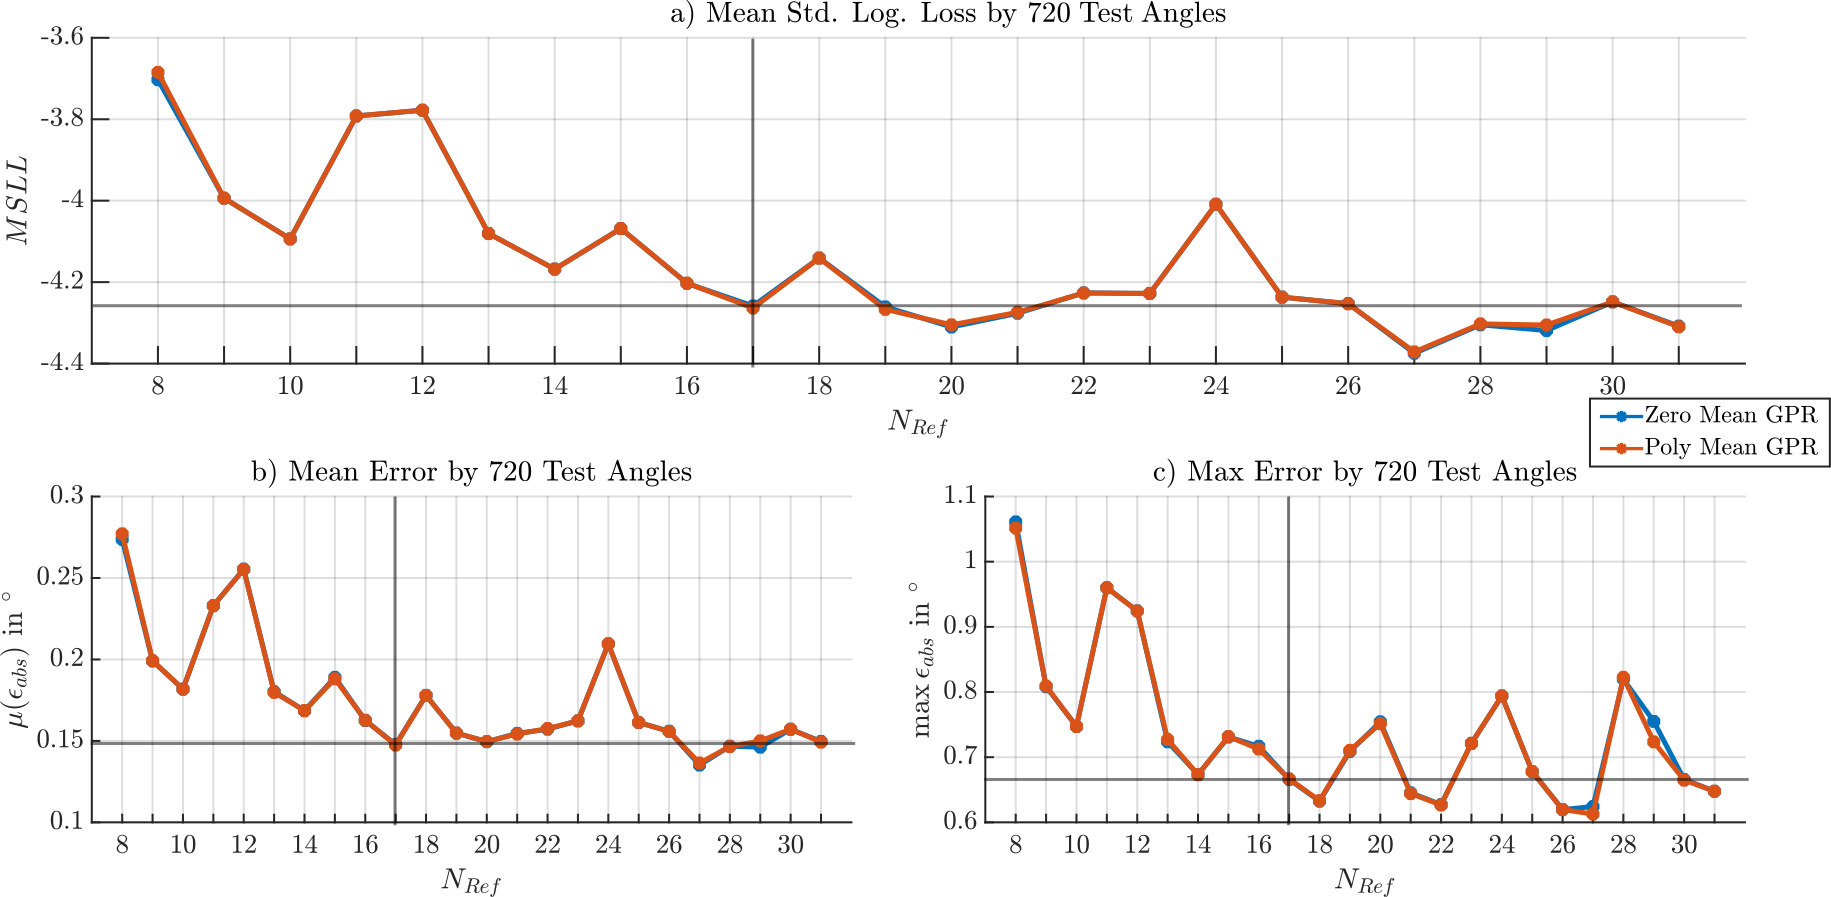
\includegraphics[width=\linewidth]{chapters/images/4-EuOExp/MSLL-vs-Errors}
	\caption[Variation der Referenzwinkelanzahl mit Optimierung des Rauschniveau]{Variation der Referenzwinkelanzahl mit Optimierung des Rauschniveaus $\sigma_n^2$ nach \autoref{alg:bayesopt}. Es wird die Implementierung des Regressionsmodell nach \autoref{eq:kfun} mit euklidischen Abstand nach \autoref{eq:de2innorm}, jeweils ohne (Zero Mean GPR) und mit Mittelwertunterstützung (Poly Mean GPR) in Abhängigkeit der Referenzwinkelanzahl $N_{Ref}$ verglichen. Dafür wird in a) die Modellgeneralisierung über den mittleren standardisierten logarithmischen Verlust (engl. Loss) $MSLL$ a. u. nach \autoref{eq:bayesopt} bewertet. Die Verlustberechnung ist für Winkelverluste konfiguriert. In b) folgen der absolute mittlere Winkelfehler sowie in c) der absolute maximale Winkelfehler. Alle drei Berechnungen sind jeweils für jeden Schritt auf eine volle Rotation durchgeführt worden. Modelltrainingsdaten basieren hier auf Vektoren bzw. Skalare.}
	\label{fig:msll-vs-errors}
\end{figure}


\clearpage

